%%%%%%%%%%%%%%%%%%%%%%%%%%%%%%%%%%%%%%%%%%%%%%%%%%%%%%%%%%%%%%%
%
% Welcome to Overleaf --- just edit your LaTeX on the left,
% and we'll compile it for you on the right. If you open the
% 'Share' menu, you can invite other users to edit at the same
% time. See www.overleaf.com/learn for more info. Enjoy!
%
%%%%%%%%%%%%%%%%%%%%%%%%%%%%%%%%%%%%%%%%%%%%%%%%%%%%%%%%%%%%%%%
%\usepgfplotslibrary{external}
%\tikzexternalize

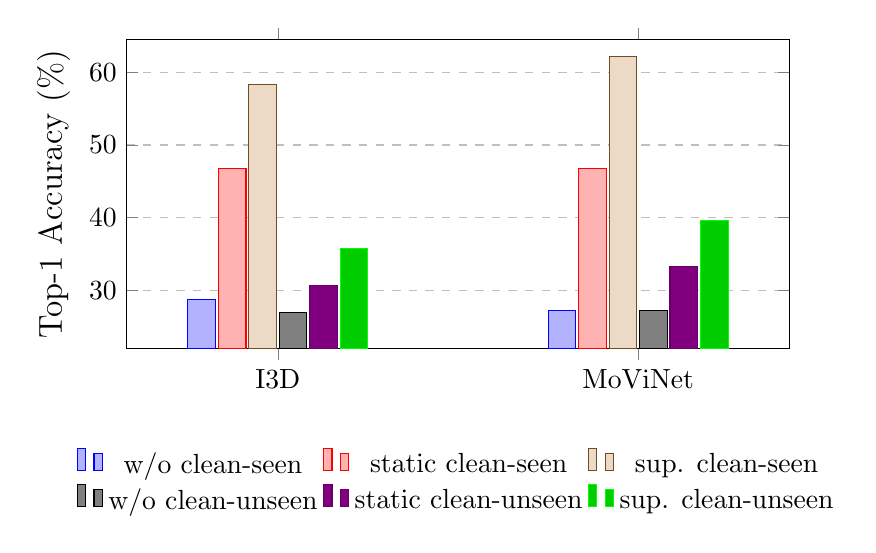
\begin{tikzpicture}
\begin{axis}[
symbolic x coords={I3D, MoViNet},
	ylabel=\large Top-1 Accuracy (\%),
	enlargelimits=false,
	ybar=1pt, enlarge x limits=0.42,
	xtick=data,
	ymin=22.0,
    ymax=64.5,
    ymajorgrids=true,
    legend style={draw=none},
          grid style=dashed,
          width=10cm,
          height=5.5cm,
         legend style={at={(0.5,-0.3)},
	    anchor=north,legend columns=3}, 
        every axis plot/.append 
        every mark/.append style={mark size=52pt}
]
\addplot 
	coordinates {
	            (I3D,28.73)
	            (MoViNet,27.20)
	};
	\addlegendentry{w/o clean-seen} 
\addplot 
	coordinates {
	            (I3D,46.77)
	            (MoViNet,46.71)
	};
	\addlegendentry{static clean-seen} 
\addplot 
	coordinates {
	            (I3D,58.33)
	            (MoViNet,62.24)
	};
	\addlegendentry{sup. clean-seen} 
	
	
	

\addplot 
	coordinates {
	            (I3D,26.96)
	            (MoViNet,27.20)
	};
	\addlegendentry{w/o clean-unseen} 

\addplot 
	coordinates {
	            (I3D,30.71)
	            (MoViNet,33.30)
	};
	\addlegendentry{static clean-unseen} 

\addplot 
	coordinates {
	            (I3D,35.71)
	            (MoViNet,39.59)
	};
	\addlegendentry{sup. clean-unseen} 

\end{axis}
\end{tikzpicture}


